% % % % % % % % % % % % % % % % % % % % % % % % % % % % % % % % % % % % % % % %
% LaTeX4EI Template for Cheat Sheets                                Version 1.1
%
% Authors: Emanuel Regnath, Martin Zellner
% Contact: info@latex4ei.de
% Encode: UTF-8, tabwidth = 4, newline = LF
% % % % % % % % % % % % % % % % % % % % % % % % % % % % % % % % % % % % % % % %


% ======================================================================
% Document Settings
% ======================================================================

% possible options: color/nocolor, english/german, threecolumn
% defaults: color, english
\documentclass[english]{latex4ei/latex4ei_sheet}

% additional packages
\DeclareTextFontCommand{\emph}{\bfseries}

% set document information
\title{How to Ace the Data Science Case Interview }
\author{LaTeX4EI}					% optional, delete if unchanged
\myemail{info@latex4ei.de}			% optional, delete if unchanged
\mywebsite{https://github.com/leoniewgnr/DataScienceCheatsheets}			% optional, delete if unchanged


% ======================================================================
% Begin
% ======================================================================
\begin{document}

\IfFileExists{git.id}{\input{git.id}}{}
\ifdefined\GitRevision\mydate{\GitNiceDate\ (git \GitRevision)}\fi

% Title
% ----------------------------------------------------------------------
\maketitle   % requires ./img/Logo.pdf


% Section
% ----------------------------------------------------------------------
\section{Understanding the Situation and Problem Statement}
\begin{sectionbox}
\begin{symbolbox}
Steps 1-4 are the steps to follow in a case interview. Step 5 gives more details on ML models.
\end{symbolbox}
    Define the business problem clearly: Take notes, repeat the problem and ask questions.\\
    Structure 
\end{sectionbox}

\section{Data Collection and Preparation}
\begin{sectionbox}
    \subsection{Data Sources}
    \begin{itemize}
        \item Databases, APIs, files
        \item Social media networks
    \end{itemize}
    What data types are those?
    
    \subsection{Data Cleaning}
    \begin{itemize}
        \item Imputation or removal
        \item Z-score: How many standard deviations a specific value is from the mean $\rightarrow > 2$ ($< -2$)
        \item IQR: Difference between Q3 and Q1 (50\% of the data), upper limit: $Q3 + 1.5 \times IQR$
    \end{itemize}
    
    \subsection{Exploratory Data Analysis (EDA)}
    \begin{itemize}
        \item Visualization: Histograms, Scatterplots, correlation matrices
        \item Statistical analysis: Distribution, trends, relationships between variables
    \end{itemize}
    
    \subsection{Data Preparation}
    \begin{itemize}
        \item Min-Max or Z-standardization
        \item Relevant features
        \item Train, val, and test split
    \end{itemize}

    \subsection{What else to consider}
    \begin{itemize}
        \item Legal: GDPR, Anonymization
        \item Scalability: Fast datatypes (dask), PCA
    \end{itemize}
\end{sectionbox}


\section{Model Selection and Development}
\begin{sectionbox}
    
\subsection{Model Selection}
\textbf{Supervised Learning}: Algorithms that learn from labeled data (e.g., Regression, Classification).\\
\textbf{Unsupervised Learning}: Algorithms that learn from unlabeled data (e.g., Clustering, Dimensionality Reduction).\\
\textbf{Reinforcement Learning}: Algorithms that learn through reward and punishment.\\
\textbf{Bias-Variance Tradeoff}: Tradeoff between overfitting (high variance) and underfitting (high bias).\\
Bias: learn the wrong relationship\\
Variance: learns random relations that do not correlate with the data

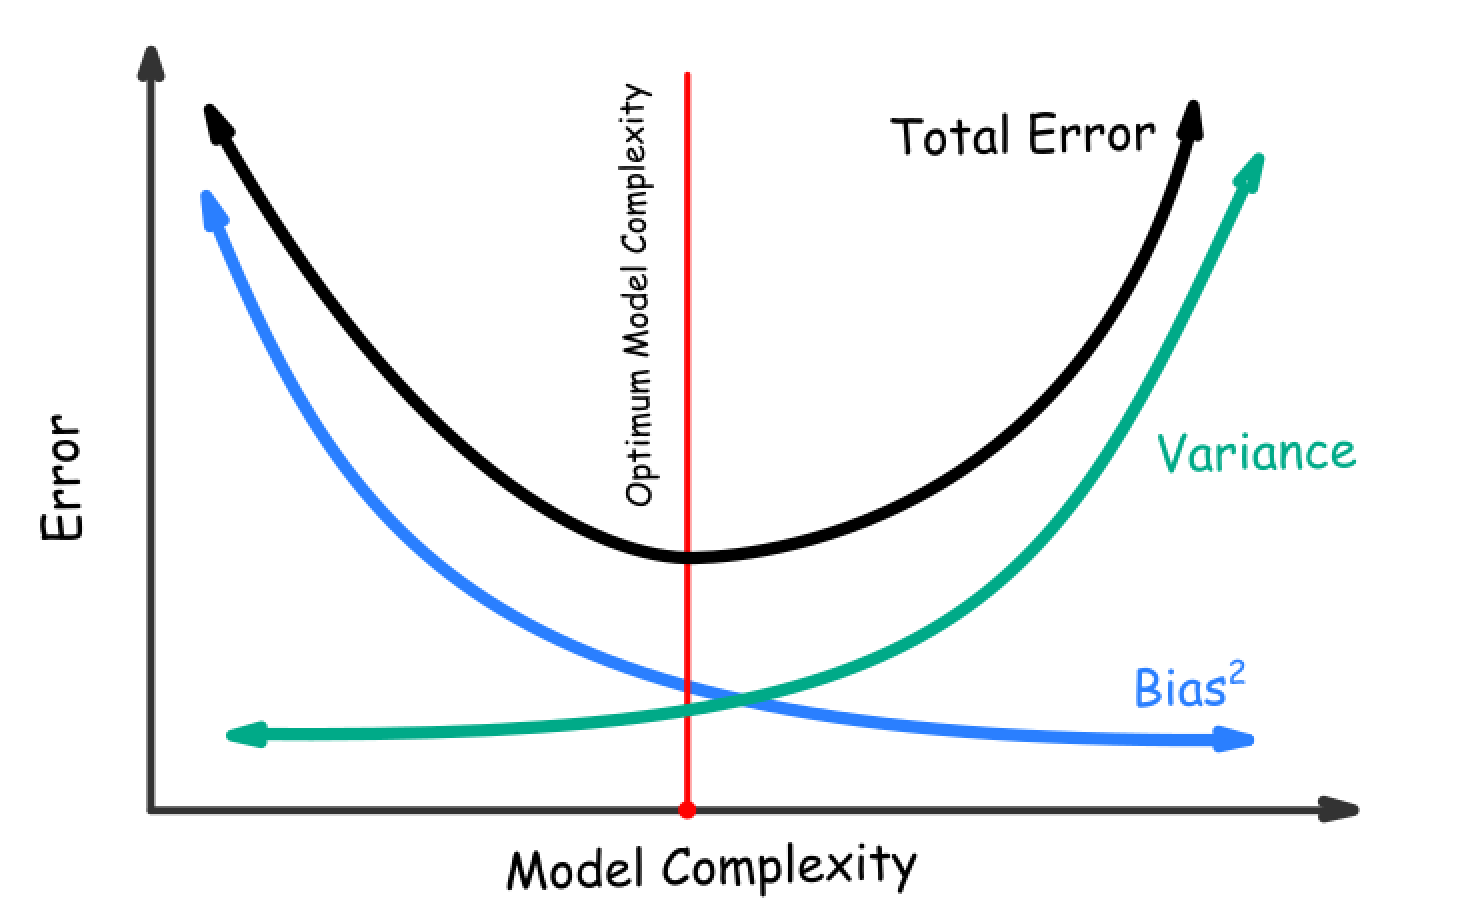
\includegraphics[width=0.5\textwidth]{cheat_sheets/img/biasvariance.png}
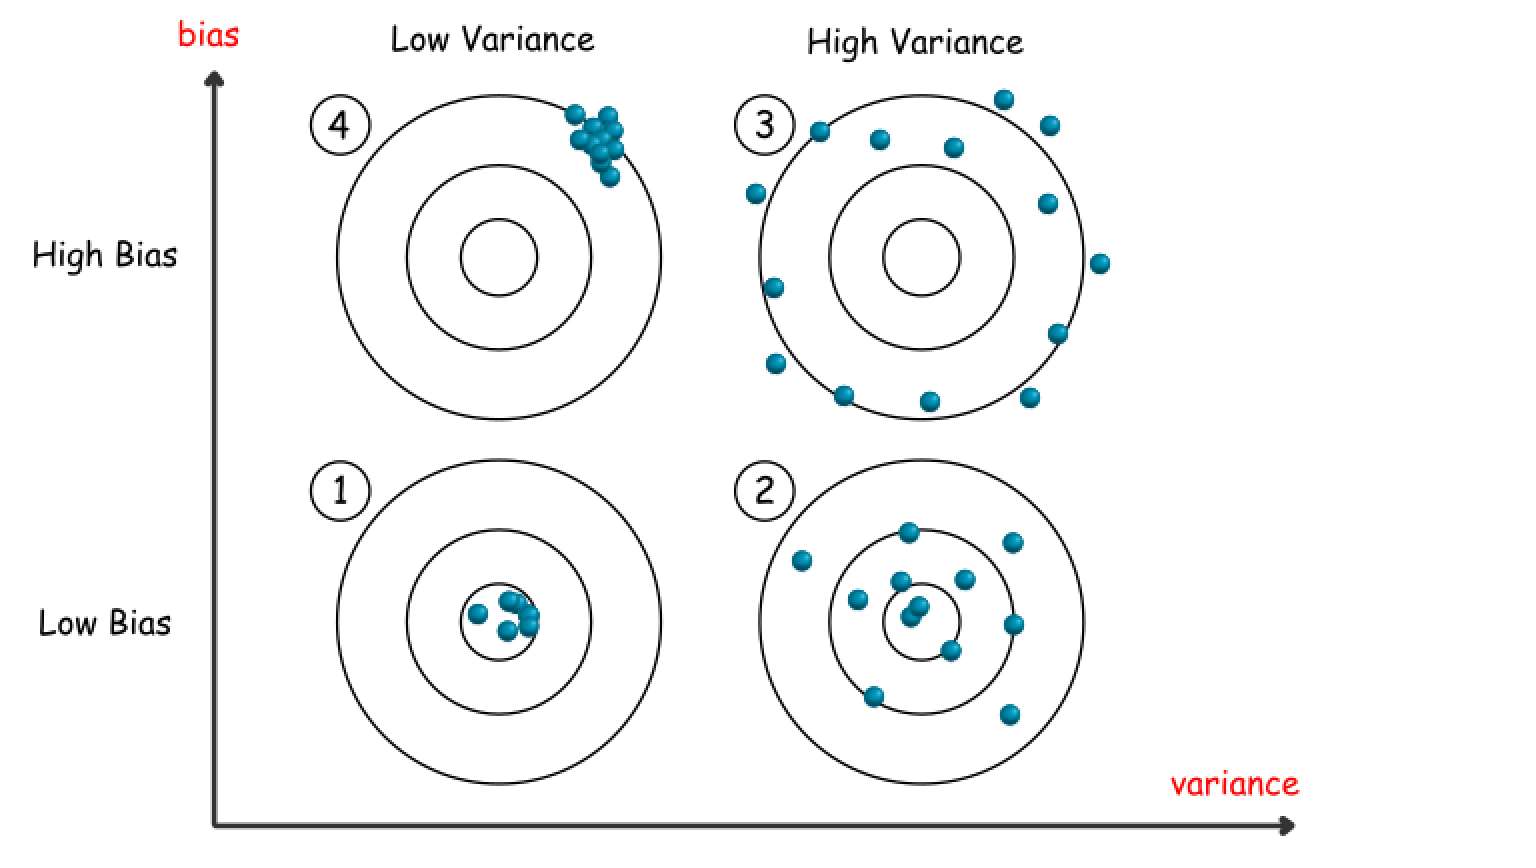
\includegraphics[width=0.5\textwidth]{cheat_sheets/img/biasmatrix.png}

\textbf{Cross-Validation:} Technique for avoiding overfitting by splitting the data into multiple folds.

\subsection{Model Development}
\textbf{Feature Engineering}: Selection and transformation of features to improve model performance.\\
\textbf{Hyperparameter Tuning}: Optimization of parameters that are not learned from the data (e.g., Learning Rate).\\
\textbf{Ensemble Learning}: Combining multiple models to improve accuracy (e.g., Random Forest, Bagging, Boosting).\\
\textbf{Regularization}: Techniques to avoid overfitting (e.g., L1/L2 regularization).\\
\textbf{Loss Functions}: Functions to measure the error of a model (e.g., Mean Squared Error, Cross-Entropy).
\end{sectionbox}

\begin{sectionbox}
\subsection{Models}
\begin{tablebox}{>\raggedright p{0.1\linewidth} >\raggedright p{0.19\linewidth} p{0.19\linewidth} p{0.19\linewidth} p{0.19\linewidth}}
& \emph{Linear Regression} & \emph{Logistic Regression} & \emph{Decision Tree} & \emph{Random Forest} \\ \cmrule
Type & Supervised & Supervised & Supervised & Supervised \\
Target Variable & Continuous & Binary/Categorical & Both & Both \\
Expl. & Linear relationship between features and target. & Estimates probabilities for categorical target variable. & Splits data based on feature values. & Ensemble of decision trees for robustness. \\
Use Case & Price prediction, Trend analysis & Classification, Spam detection & Classification, Regression & Classification, Regression \\
Prereqs. & Linear relationship & Linear boundaries & None & None \\
Complex. & Low & Low & Medium & Medium \\
Params & Learning rate, Regularization & Learning rate, Regularization & Depth, Split criteria & Number of trees, Depth \\
Metric & RMSE, MAE & Accuracy, F1 & Accuracy, RMSE & Accuracy, RMSE \\
Interpret- ability & High & High & Medium & Medium \\
\end{tablebox}

\begin{tablebox}{>\raggedright p{0.1\linewidth} >\raggedright p{0.19\linewidth} p{0.19\linewidth} p{0.19\linewidth} p{0.19\linewidth}}
& \emph{SVM} & \emph{K-NN} & \emph{K-Means} & \emph{Neural Networks} \\ \cmrule
Type & Supervised & Supervised & Unsupervised & Supervised \\
Target Variable & Binary/Categorical & Both & None & Both \\
Expl. & Finds the best separating line/plane between classes. & Classifies elements based on their neighbors. & Groups data into k similar clusters. & Simulates a neural network for complex patterns. \\
Use Case & Text classification, Face recognition & Recommendation systems, Classification & Customer segmentation, Anomaly detection & Image recognition, NLP \\
Prereqs. & Scaling, Labeling & Feature scaling & None & Large data set \\
Complex. & High & Low & Medium & High \\
Params & C, Kernel & Number of neighbors & Number of clusters & Learning rate, Neurons, Layers \\
Metric & Accuracy, F1 & Accuracy, RMSE & Silhouette Score, Inertia & Accuracy, F1 \\
Interpret- ability & Low & High & Medium & Low \\
\end{tablebox}

\begin{tablebox}{>\raggedright p{0.1\linewidth} >\raggedright p{0.39\linewidth} p{0.39\linewidth}}
& \emph{Naive Bayes} & \emph{ARIMA} \\ \cmrule
Type & Supervised & Supervised \\
Target Variable & Categorical & Time series \\
Expl. & Uses Bayesian theory for classification. & Models time series through trend, seasonality, and noise. \\
Use Case & Text classification, Spam filter & Financial markets, Weather prediction \\
Prereqs. & Independent features & Stationarity \\
Complex. & Low & Medium \\
Params & Laplace smoothing & p, d, q parameters \\
Metric & Accuracy, F1 & RMSE, MAE \\
Interpret- ability & High & Medium \\
\end{tablebox}
\end{sectionbox}

\begin{sectionbox}
\subsection{Evaluation Metrics}
\subsubsection{Regression}
\textbf{Mean Squared Error (MSE)} $\frac{1}{n}\sum (y_i - \hat{y_i})^2$\\
\textbf{Sum of Squared Errors (SSE)} $\sum (y_i - \hat{y_i})$\\
\textbf{Total Sum of Squares (SST)} $\sum (y_i - \overline{y_i})$\\

\subsubsection{Metrics}
\textbf{Accuracy}: Ratio of correct predictions to the total number of predictions. BUT: problem with imbalanced classes $\rightarrow$ good for classification problems with balanced classes\\
\textbf{Precision}: $\frac{TP}{TP+FP}$ $\rightarrow$ideal if no FP (Spam detection: negative/no-spam mail is detected as positive/spam)\\
\textbf{Recall (TPR)}: $\frac{TP}{TP+FN}$ $\rightarrow$ ideal if no FN (Disease detection: positive/sick patient is detected as healthy/negative)\\
\textbf{F1-Score}: $2\frac{\text{precision} * \text{recall}}{\text{precision} + \text{recall}}$ $\rightarrow$ for imbalanced classes\\
\textbf{ROC-AUC}: Plot TPR vs FPR for different classification thresholds, aread under the curve = how likely the model differentiates positives vs negatives (1: perfect classification, 0.5: like random), not dependent on threshold, not always interpretable\\
\textbf{$R^2$ Score}: $1-\frac{SSE}{SST}$ ratio of explained variability in the data, not valid for nonlinear models \\


% Image is included as a placeholder
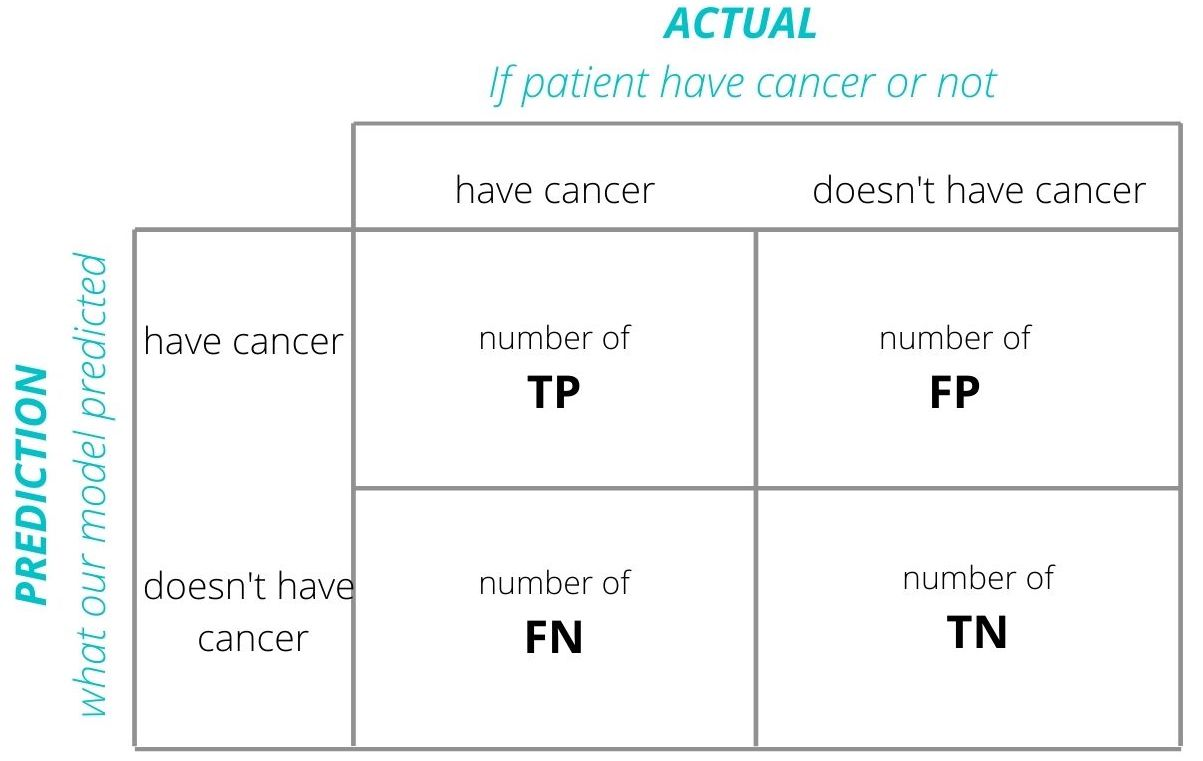
\includegraphics[width=0.5\textwidth]{cheat_sheets/img/confusion.jpeg}

\end{sectionbox}

\section{Implementation and Communication}
\begin{sectionbox}
\subsection{Implementation}
    \textbf{Version Control (e.g., Git)}: For collaborative work and tracking changes.\\
    \textbf{Continuous Integration / Continuous Deployment (CI/CD)}: Automatic testing and deployment of code.\\
    \textbf{Model Serving}: Hosting models for real-time access, e.g., via REST APIs.
    \item \textbf{Containerization (e.g., Docker)}: Packaging of software and dependencies for consistent execution.\\
    \textbf{Scaling}: Adjusting resources to load, e.g., through horizontal scaling.\\
    \textbf{Monitoring \& Logging}: Monitoring system performance and capturing important information.
        
\subsection{Communication}
    \textbf{Data Visualization}: Effective presentation of data using charts (e.g., Matplotlib, Seaborn).\\
    \textbf{Storytelling with Data}: Connecting analyses with a narrative structure to convey insights.\\
    \textbf{Interactive Dashboards (e.g., Tableau, Power BI, Dash)}: Creating interactive reports for end users.\\
    \textbf{Technical Documentation}: Clear and precise documentation of code, architecture, and decisions.\\
    \textbf{Non-Technical Communication}: Explaining technical concepts to a broader audience (e.g., stakeholders).\\
        \begin{itemize}
            \item ROI Analysis (Return on Investment): Evaluating how the results affect the business outcome.
            \item KPIs (Key Performance Indicators): Understanding and measuring the key metrics relevant to the business goal.
            \item Statistical Significance \& Confidence Intervals: Assessing the reliability of the results.
            \item Cost-Benefit Analysis: Weighing the implementation costs against expected benefits.
            \item Risk Assessment: Assessing potential risks or downsides of implementing the results.
            \item Scenario Analysis: Conducting "what-if" analyses to understand different business scenarios.
        \end{itemize}
    \textbf{Ethics and Compliance}: Understanding and adhering to legal and ethical guidelines (e.g., GDPR).
    
\subsection{Model Management}
    \textbf{Model Tracking (e.g., MLflow)}: Tracking experiments, models, and metrics.\\
    \textbf{A/B Testing}: Comparing model versions to select the best.\\
\end{sectionbox}

\section{Machine Learning Models}
\begin{sectionbox}
\subsection{Linear Regression}
Most basic and widely used techniques in predictive modeling\\
linear relationship between the dependent variable and one or more independent continuous variables
\subsubsection{Assumptions}
\begin{itemize}
    \item Linear Relationship: Assumes that the relationship between the dependent and independent variables is linear.
    \item Independence: Observations are independent of each other.
    \item Homoscedasticity: Constant variance of errors.
    \item Normality: The errors follow a normal distribution.
\end{itemize}

\subsubsection{Equation}
\(y = \beta_0 + \beta_1 x_1 + \epsilon\), where \(y\) is the dependent variable, \(x_1\) is the independent variable, \(\beta_0\) is the y-intercept, \(\beta_1\) is the slope, and \(\epsilon\) is the error term.

\subsubsection{Training Parameters}
Learning Rate: For gradient descent optimization.\\
Regularization: To prevent overfitting.
\begin{itemize}
    \item Ridge Regularization (L2): $\|Y-X \beta\|^{2}+\lambda\|\beta\|^{2}$ $\rightarrow$ coefficients to almost zero (keeps all features), less computationally complex, better if predictors are highly correlated
    \item Lasso Regularization (L1): $\|Y-X \beta\|^{2}+\lambda\|\beta\|_{1}$ $\rightarrow$ some coefficients to zero (feature selection)
    \item Elastic net: combined
\end{itemize}

\subsubsection{Use-cases}
\begin{itemize}
    \item Price prediction
    \item Trend forecasting
    \item Risk assessment
\end{itemize}

\begin{tablebox}{p{0.4\textwidth} p{0.55\textwidth}}
\emph{Strengths} & \emph{Weaknesses} \\ \cmrule
Simple and interpretable &  Only captures linear relationships\\
Fast to model and predict & Sensitive to outliers\\
Works well on small datasets & Cannot handle multicollinearity (independent variables are highly correlated) well\\
\end{tablebox}

\subsubsection{Data Preprocessing}
\begin{itemize}
    \item Feature scaling: Often required.
    \item Missing values: Need to be handled.
    \item Categorical variables: One-Hot Encoding.
\end{itemize}

\subsubsection{Interpretability}
High; coefficients represent the change in the dependent variable for a one-unit change in an independent variable.

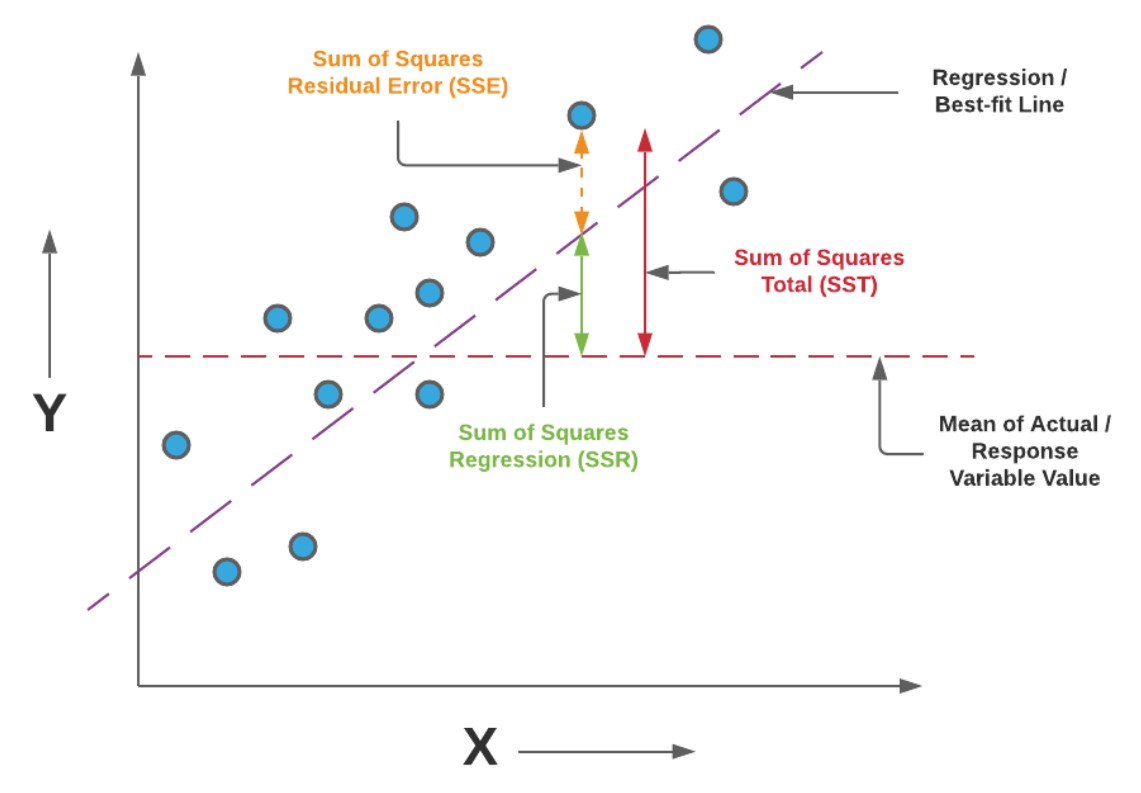
\includegraphics[width=0.6\linewidth]{cheat_sheets//img/linear-regression-f-statistics-definition.jpg}
\end{sectionbox}

\begin{sectionbox}
\subsection{Logistic Regression}
for classification problems, especially for binary outcomes\\
Transforms its output to lie in the range of 0 to 1 using the logistic function.

\subsubsection{Assumptions}
\begin{itemize}
    \item Linear Relationship: Assumes a linear relationship between the logit of the outcome and the predictor variables.
    \item Independence: Observations should be independent of each other.
    \item Large Sample Size: Needs a large sample size for maximum likelihood estimates to be truly asymptotic.
\end{itemize}

\subsubsection{Equation}
\( \ln\left(\frac{p}{1-p}\right) = \beta_0 + \beta_1 x_1 + \epsilon \), where \( p \) is the probability of the dependent event occurring, \( x_1 \) is the independent variable, \( \beta_0 \) is the intercept, \( \beta_1 \) is the slope, and \( \epsilon \) is the error term.

\subsubsection{Training Parameters}
\begin{itemize}
    \item Learning Rate: For optimization using methods like stochastic gradient descent.
    \item Regularization: To avoid overfitting, commonly used methods include L1 and L2 regularization.
\end{itemize}

\subsubsection{Use-cases}
\begin{itemize}
    \item Customer churn prediction
    \item Image classification
    \item Medical diagnosis
\end{itemize}

\begin{tablebox}{p{0.4\textwidth} p{0.55\textwidth}}
\emph{Strengths} & \emph{Weaknesses} \\ \cmrule
High interpretability & Not suitable for non-linear problems \\
Efficient to train & Sensitive to feature scale \\
Can provide calibrated probabilities & Prone to underfitting \\
\end{tablebox}

\subsubsection{Data Preprocessing}
\begin{itemize}
    \item Feature Scaling: Required for regularization and gradient descent.
    \item Missing Values: Must be addressed.
    \item Categorical Variables: Label encoding or one-hot encoding often used.
\end{itemize}

\subsubsection{Interpretability}
Coefficients signify the odds ratio for the given predictor variable. A coefficient greater than 1 represents increased odds of the outcome, while a coefficient less than 1 represents decreased odds.

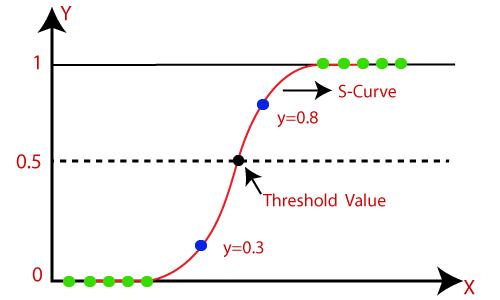
\includegraphics[width=0.5\linewidth]{cheat_sheets//img/logistic-regression-in-machine-learning.png}
\end{sectionbox}

\begin{sectionbox}
    \subsection{Decision Tree}
For both classification and regression tasks. \\
Decision trees work by splitting the dataset into subsets based on the most significant attributes, making decisions at every level.

\subsubsection{Assumptions}
\begin{itemize}
    \item None: One of the few algorithms that does not assume any underlying data distribution.
\end{itemize}

\subsubsection{Equation}
No single equation represents a decision tree. They are built using algorithms like ID3, C4.5, or CART, which use measures like Information Gain, Gain Ratio, or Gini Index to decide splits.

\subsubsection{Training Parameters}
\begin{itemize}
    \item Max Depth: Maximum depth of tree.
    \item Min Samples Split: Minimum number of samples required to split an internal node.
    \item Min Samples Leaf: Minimum number of samples required to be at a leaf node.
    \item Criterion: Metric used for splitting (Gini, Entropy).
\end{itemize}

\subsubsection{Use-cases}
\begin{itemize}
    \item Customer segmentation
    \item Fraud detection
    \item Medical diagnosis
\end{itemize}

\begin{tablebox}{p{0.4\textwidth} p{0.55\textwidth}}
\emph{Strengths} & \emph{Weaknesses} \\ \cmrule
High interpretability & Sensitive to noisy data \\
Can handle both categorical and numerical data & Prone to overfitting \\
No assumptions about data & Not suitable for unstructured data like images, text \\
\end{tablebox}

\subsubsection{Data Preprocessing}
\begin{itemize}
    \item Feature Scaling: Not required.
    \item Missing Values: Can be handled but better to address.
    \item Categorical Variables: Label encoding sufficient, though one-hot can be used.
\end{itemize}

\subsubsection{Interpretability}
High; each node represents a decision based on one attribute, and the path from root to leaf gives the reasoning for the final decision.

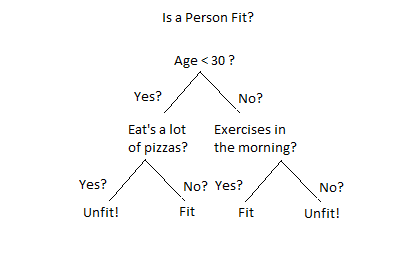
\includegraphics[width=0.5\linewidth]{cheat_sheets//img/Decision-Trees-modified-1.png}
\end{sectionbox}

\begin{sectionbox}
\subsection{Random Forests}
An ensemble learning method that combines multiple decision trees to create a more robust and accurate model\\
For both classification and regression tasks.

\subsubsection{Assumptions}
\begin{itemize}
    \item None: Like Decision Trees
\end{itemize}

\subsubsection{Architecture}
collections of decision trees
\begin{itemize}
    \item \textbf{Bagging (Bootstrap Aggregating)}: Each tree is trained on a different subset of data, subsets are created by sampling with replacement $\rightarrow$ diversity among trees and minimize overfitting\\
    1. Take a boostrap sample from training data; 2. Build decision tree using this sample
    \item \textbf{Feature Randomness}: standard decision tree: each node, consider all features to find best split $\leftrightarrow$ Random Forest: at each node only a random subset of features, best feature from this subset is used to make the split $\rightarrow$ diversity among trees and more robust
\end{itemize}

\subsubsection{Training Parameters}
\begin{itemize}
    \item Number of Trees: The more trees, the less likely the model will overfit.
    \item Same as decision tree
\end{itemize}

\subsubsection{Use-cases}
\begin{itemize}
    \item Predictive Maintenance
    \item Recommendation Systems
    \item Financial Modeling
\end{itemize}

\begin{tablebox}{p{0.4\textwidth} p{0.55\textwidth}}
\emph{Strengths} & \emph{Weaknesses} \\ \cmrule
High accuracy & Computationally expensive \\
Low overfitting risk & Less interpretable compared to a single decision tree \\
Handles unbalanced datasets well & Not ideal for real-time predictions \\
\end{tablebox}

\subsubsection{Data Preprocessing}
\begin{itemize}
    \item Feature Scaling: Generally not required.
    \item Missing Values: Can handle missing values, but better to impute.
    \item Categorical Variables: Label encoding usually sufficient.
\end{itemize}

\subsubsection{Interpretability}
Moderate; while individual trees are interpretable, the ensemble model complicates interpretation. However, feature importance can still be extracted.
\end{sectionbox}

\begin{sectionbox}
\subsection{Support Vector Machine (SVM)}

Effective for both linear and non-linear classification, regression, and outlier detection.

\subsubsection{Assumptions}
\begin{itemize}
    \item No Noise: Assumes that the data is clean and that there are clear margins of separation.
    \item Two Classes: For basic SVM, the algorithm is inherently binary.
\end{itemize}

\subsubsection{Equation}
The objective is to maximize the margin, defined by \( \frac{2}{\|w\|} \), where \(w\) is the weight vector, subject to constraints \( y_i(w \cdot x_i + b) \geq 1 \).

\subsubsection{Training Parameters}
Kernel: Specifies the type of hyperplane used to separate the data.
\begin{itemize}
    \item Linear Kernel: \(K(x, y) = x \cdot y\)
    \item Polynomial Kernel: \(K(x, y) = (1 + x \cdot y)^d\)
    \item RBF Kernel: \(K(x, y) = e^{-\gamma ||x-y||^2}\)
\end{itemize}
Regularization (C parameter): Balances classification and margin maximization. 

\subsubsection{Use-cases}
\begin{itemize}
    \item Text classification
    \item Image recognition
    \item Bioinformatics (e.g., cancer classification)
\end{itemize}

\begin{tablebox}{p{0.4\textwidth} p{0.55\textwidth}}
\emph{Strengths} & \emph{Weaknesses} \\ \cmrule
High accuracy & Computationally expensive \\
Good for high-dimensional spaces & Sensitive to choice of kernel and regularization \\
Handles non-linear data well & Difficult to interpret \\
\end{tablebox}

\subsubsection{Data Preprocessing}
\begin{itemize}
    \item Feature scaling: Essential due to distance-based optimization.
    \item Missing values: Must be handled prior.
    \item Categorical variables: Ordinal Encoding or One-Hot Encoding.
\end{itemize}

\subsubsection{Interpretability}
Low; the model parameters are hard to interpret in the context of the data, especially for non-linear kernels.

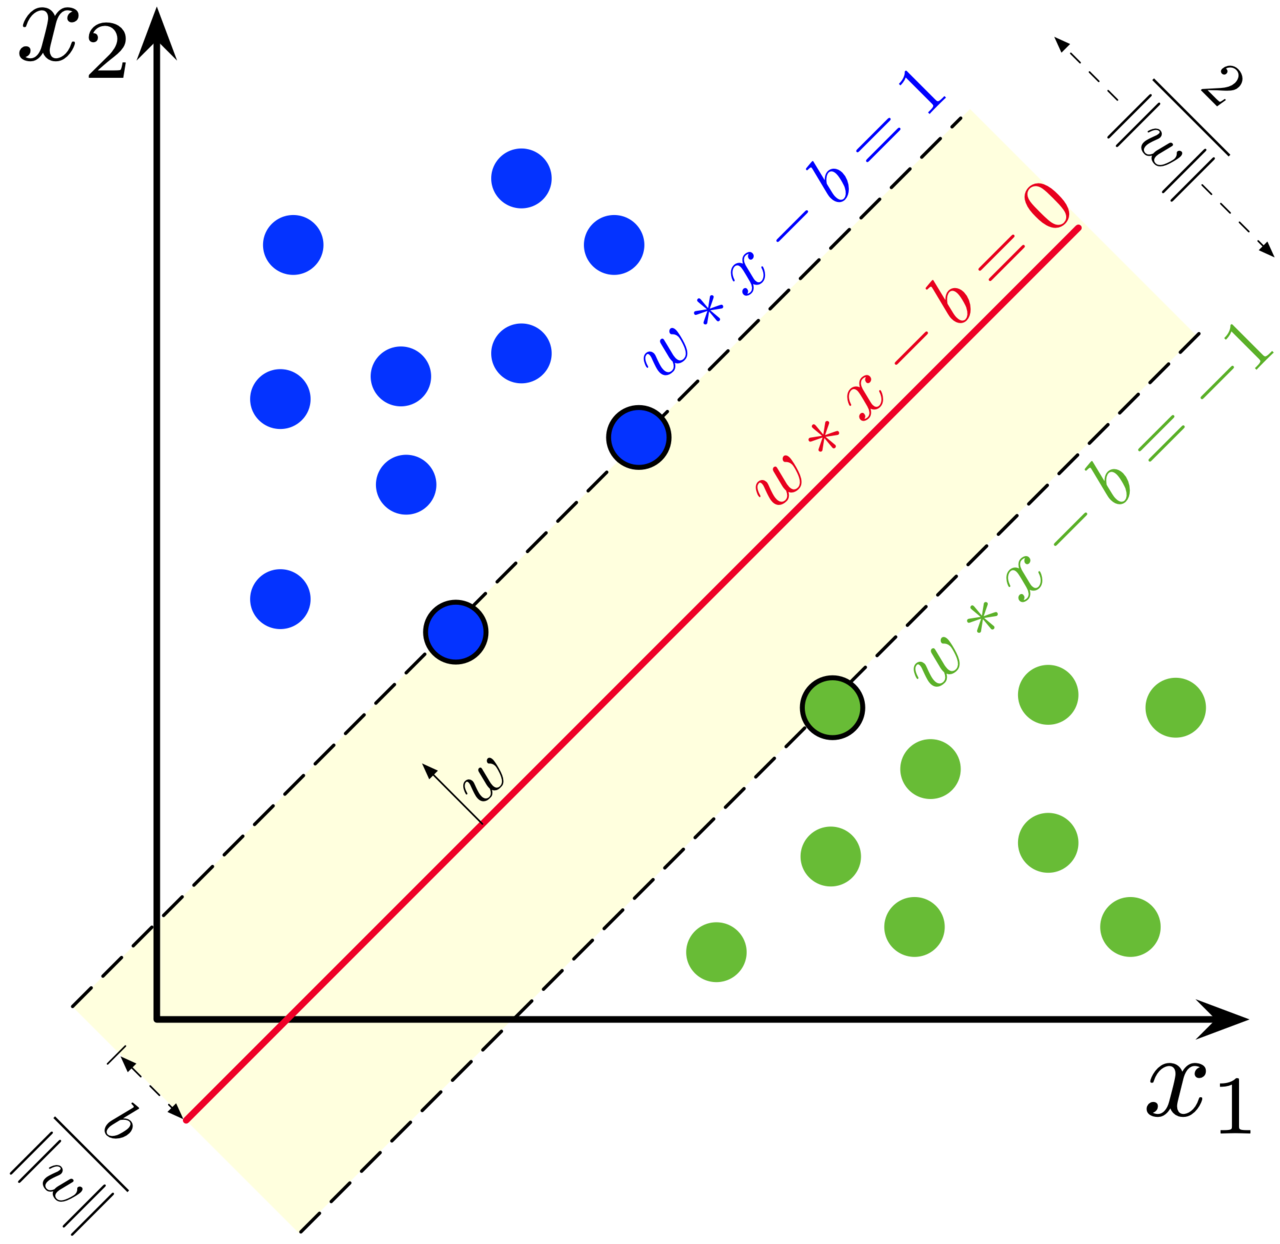
\includegraphics[width=0.3\linewidth]{cheat_sheets//img/1280px-SVM_margin.png}
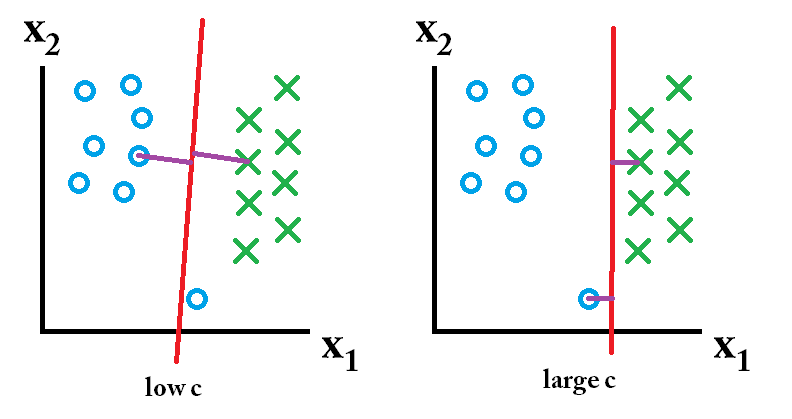
\includegraphics[width=0.5\linewidth]{GbW5S.png}
\end{sectionbox}

\begin{sectionbox}
\subsection{k-Nearest Neighbors (k-NN)}

A non-parametric method used for classification and regression tasks based on similarity measures.

\subsubsection{Assumptions}
\begin{itemize}
    \item No underlying model: Assumes no prior knowledge about the underlying data distribution.
    \item Similarity Measure: Assumes similar instances are near each other in the feature space.
\end{itemize}

\subsubsection{Architecture}
Classification is performed by a majority vote among the k-nearest points. Distance measures can include Euclidean, Manhattan, etc.

\subsubsection{Training Parameters}
\begin{itemize}
    \item \( k \): Number of neighbors to consider.
    \item Distance Metric: How to measure the distance between points (e.g., Euclidean, Manhattan).
    \item Weighting: Assign weights to contributions of the neighbors.
\end{itemize}

\subsubsection{Use-cases}
\begin{itemize}
    \item Text categorization
    \item Fraud detection
    \item Recommender systems
\end{itemize}

\begin{tablebox}{p{0.4\textwidth} p{0.55\textwidth}}
\emph{Strengths} & \emph{Weaknesses} \\ \cmrule
Simple to implement & Computationally expensive \\
Adapts easily to multi-class problems & Sensitive to irrelevant features \\
Effective if the feature dimension is low & Requires meaningful distance function \\
\end{tablebox}

\subsubsection{Data Preprocessing}
\begin{itemize}
    \item Feature scaling: Crucial because k-NN uses distance measures.
    \item Missing values: Must be handled; otherwise, they'll impact distance calculations.
    \item Categorical variables: Ordinal Encoding or One-Hot Encoding.
\end{itemize}

\subsubsection{Interpretability}
Moderate; results can be interpreted by examining the closest neighbors, though this becomes harder as dimensionality increases.
\end{sectionbox}

\begin{sectionbox}
\subsection{K-Means Clustering}
An unsupervised learning technique for partitioning data into clusters based on similarity.

\subsubsection{Assumptions}
\begin{itemize}
    \item Distance Metric: Assumes Euclidean distance as a similarity measure.
    \item Spherical Clusters: Assumes clusters to be spherical and equally sized.
\end{itemize}

\subsubsection{Equation}
Objective is to minimize the sum of squared distances from each point to its cluster centroid.

\[
J = \sum_{i=1}^{k} \sum_{x \in C_i} \|x - \mu_i\|^2
\]

where \(J\) is the objective function, \(C_i\) is the \(i^{th}\) cluster, and \(\mu_i\) is the centroid of \(C_i\).

\subsubsection{Training Parameters}
\begin{itemize}
    \item \( k \): Number of clusters.
    \item Initialization: Method for initializing centroids (e.g., random, k-means++).
    \item Max Iterations: Maximum number of iterations for the algorithm to run.
    \item Tolerance: Convergence criteria.
\end{itemize}

\subsubsection{Use-cases}
\begin{itemize}
    \item Market segmentation
    \item Document clustering
    \item Anomaly detection
\end{itemize}

\begin{tablebox}{p{0.4\textwidth} p{0.55\textwidth}}
\emph{Strengths} & \emph{Weaknesses} \\ \cmrule
Simple and fast & Must specify \( k \) in advance \\
Works well for spherical clusters & Sensitive to initial conditions \\
Easily interpretable & Struggles with different cluster sizes \\
\end{tablebox}

\subsubsection{Data Preprocessing}
\begin{itemize}
    \item Feature scaling: Important due to the use of distance metrics.
    \item Missing values: Need to be handled.
\end{itemize}

\subsubsection{Interpretability}
High; centroids and clusters can be easily examined, but interpretation can be subjective.

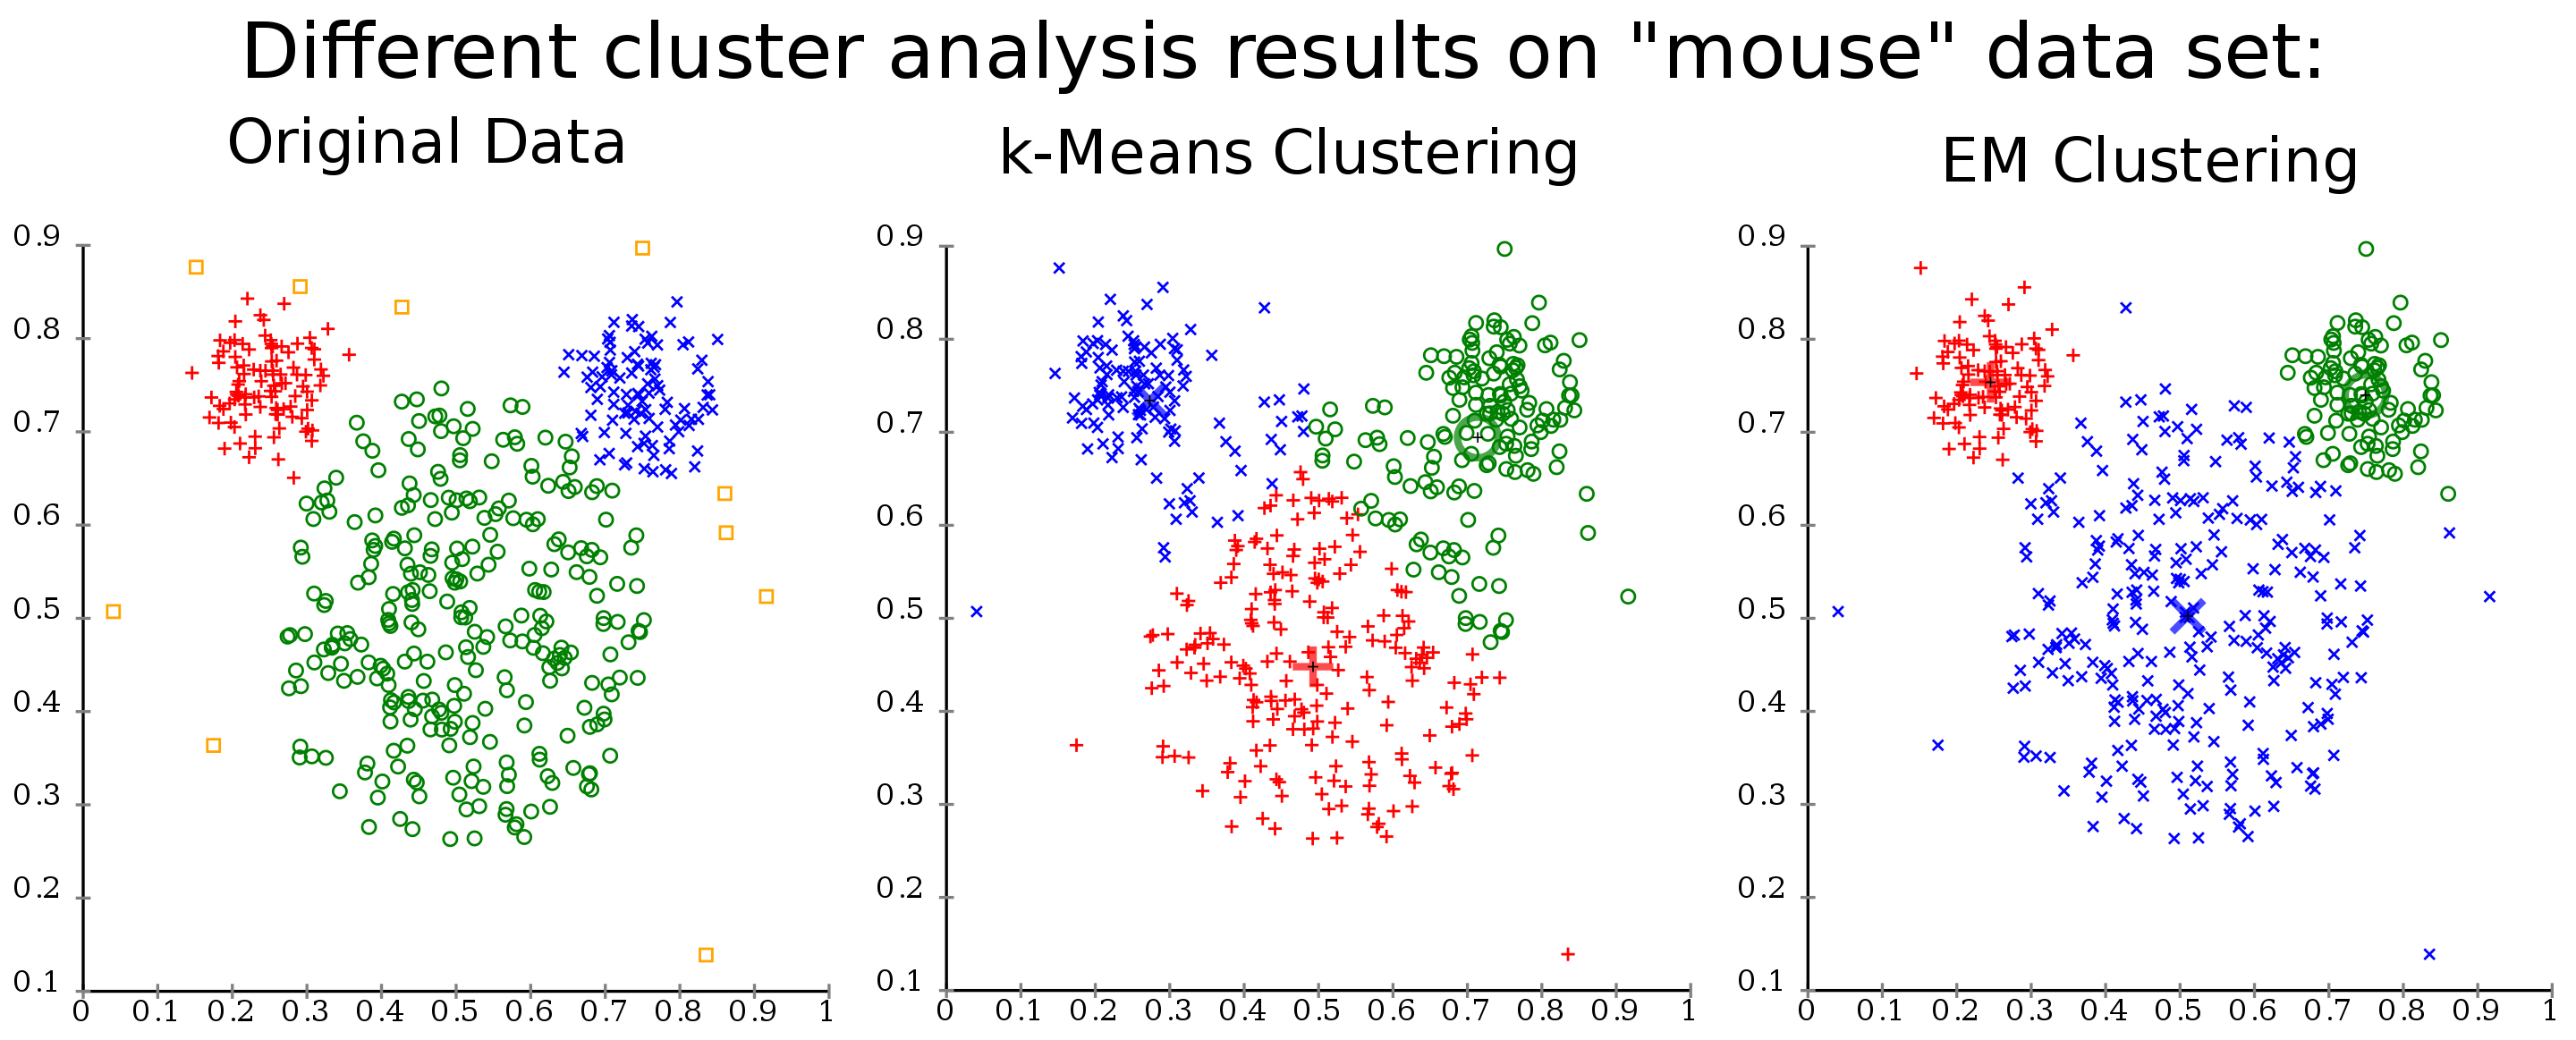
\includegraphics[width=0.9\linewidth]{2880px-ClusterAnalysis_Mouse.svg.png}
\end{sectionbox}

\begin{sectionbox}
\subsection{Neural Networks}

A class of models inspired by biological neural networks, mainly used for complex pattern recognition and nonlinear function approximation.

\subsubsection{Assumptions}
\begin{itemize}
    \item Universality: Capable of approximating any function given enough neurons.
    \item Data-Driven: Does not impose explicit assumptions on the underlying data distribution.
\end{itemize}

\subsubsection{Equation}
A typical layer in a neural network is defined as:

\[
h = \sigma(Wx + b)
\]

where \( h \) is the output, \( \sigma \) is the activation function, \( W \) is the weight matrix, \( x \) is the input, and \( b \) is the bias.

\subsubsection{Training Parameters}
\begin{itemize}
    \item Learning Rate: Step size in optimization algorithm.
    \item Activation Function: ReLU, Sigmoid, Tanh, etc.
    \item Epochs: Number of times the entire dataset is passed through the network.
    \item Batch Size: Number of samples used in each update.
\end{itemize}

\subsubsection{Use-cases}
\begin{itemize}
    \item Image classification
    \item Natural language processing
    \item Game playing
\end{itemize}

\begin{tablebox}{p{0.4\textwidth} p{0.55\textwidth}}
\emph{Strengths} & \emph{Weaknesses} \\ \cmrule
Highly flexible & Requires large data sets \\
Good for complex tasks & Computationally intensive \\
Self-learning features & Difficult to interpret \\
\end{tablebox}

\subsubsection{Data Preprocessing}
\begin{itemize}
    \item Feature scaling: Generally required.
    \item Missing values: Not well-suited; must be handled externally.
\end{itemize}

\subsubsection{Interpretability}
Low; often considered as "black-box" models due to their complex structure.
\end{sectionbox}

\begin{sectionbox}
\subsection{Naive Bayes}

Probabilistic classifiers based on Bayes' theorem, with strong independence assumptions between features.

\subsubsection{Assumptions}
\begin{itemize}
    \item Conditional Independence: Assumes that features are conditionally independent given the class label.
    \item Prior Probability: Requires an estimate of the prior probability of each class.
\end{itemize}

\subsubsection{Equation}
The posterior probability for a class \( C \) given features \( x_1, x_2, \ldots, x_n \) is:
\[
P(C|x_1, x_2, \ldots, x_n) \propto P(C) \prod_{i=1}^{n} P(x_i|C), 
\]
where $P(C)$ is the prior of class C and $P(x_i|C)$ the likelihood

\subsubsection{Training Parameters}
\begin{itemize}
    \item Smoothing: Additive smoothing (Laplace or Lidstone).
    \item Feature Type: Multinomial, Gaussian, or Bernoulli.
\end{itemize}

\subsubsection{Use-cases}
\begin{itemize}
    \item Spam filtering
    \item Sentiment analysis
    \item Document classification
\end{itemize}

\begin{tablebox}{p{0.4\textwidth} p{0.55\textwidth}}
\emph{Strengths} & \emph{Weaknesses} \\ \cmrule
Simple and fast & Assumes feature independence \\
Works well with high dimensions & Sensitive to irrelevant features \\
Effective with small data & Limited to categorical data \\
\end{tablebox}

\subsubsection{Data Preprocessing}
\begin{itemize}
    \item Feature selection: Useful to remove irrelevant features.
    \item Data transformation: Often required for Gaussian Naive Bayes.
\end{itemize}

\subsubsection{Interpretability}
High; easily understandable probabilities and strong assumptions make the model interpretable.
\end{sectionbox}

\begin{sectionbox}
\subsection{ARIMA}

AutoRegressive Integrated Moving Average (ARIMA) is a popular time-series forecasting method.

\subsubsection{Assumptions}
\begin{itemize}
    \item Stationarity: Assumes the data is stationary or can be made stationary through differencing.
    \item Linearity: Assumes a linear relationship between lagged variables.
\end{itemize}

\subsubsection{Equation}
The ARIMA model can be represented as ARIMA\((p, d, q)\), where \(p\) is the AR term, \(d\) is the number of differencing required to make the series stationary, and \(q\) is the MA term.

\[
(1 - \Phi_{1}B - \ldots - \Phi_{p}B^{p}) (1 - B)^{d} Y_{t} = (1 + \theta_{1}B + \ldots + \theta_{q}B^{q}) \epsilon_{t}
\]

\subsubsection{Training Parameters}
\begin{itemize}
    \item \(p\): Number of AR (AutoRegressive) terms.
    \item \(d\): Order of differencing.
    \item \(q\): Number of MA (Moving Average) terms.
\end{itemize}

\subsubsection{Use-cases}
\begin{itemize}
    \item Stock price forecasting
    \item Sales prediction
    \item Weather forecasting
\end{itemize}

\begin{tablebox}{p{0.4\textwidth} p{0.55\textwidth}}
\emph{Strengths} & \emph{Weaknesses} \\ \cmrule
Effective for univariate time-series & Sensitive to parameter choices \\
Handles seasonality with SARIMA & Requires stationary data \\
Good interpretability & Complexity increases with parameters \\
\end{tablebox}

\subsubsection{Data Preprocessing}
\begin{itemize}
    \item Seasonal decomposition: For seasonal data.
    \item Differencing: To achieve stationarity.
\end{itemize}

\subsubsection{Interpretability}
Moderate; understanding the parameters and their impact on the time series provides some level of interpretability.

\end{sectionbox}
% ======================================================================
% End
% ======================================================================
\end{document}
